\documentclass[twocolumn,11pt]{extarticle}
\usepackage[top=25mm, right=25mm, left=25mm, bottom=25mm]{geometry}
\usepackage{graphicx} % Required for inserting images
\usepackage{lscape}
\usepackage{float}
\usepackage{hyperref}
\usepackage[utf8]{inputenc}
\usepackage[
backend=biber,
style=ieee,
sorting=ynt,
urldate=iso8601
]{biblatex}

\addbibresource{mybib.bib}


\title{\vspace{-2cm}Revisiting ``A Synthetic Recipe for OCR'': a case study in Pashto}
\author{Final report for LT2926,  Machine learning for statistical NLP: advanced (H24)}
\date{}

\begin{document}

\maketitle

\section{Introduction}  

This report documents my final project for LT2926. I use synthetic data to train OCR models for Pashto, a low-resource language, and evaluate the performance of those trained models on a real-life Pashto dataset. 

\section{Motivation}

NLP for low-resource languages is a challenging task, in large part due to (as the name suggests) a dearth of data to train and evaluate models. \cite{magueresse_low-resource_2020}.

While working on the first assignment, I became curious by the question of how Optical Character Recognition (OCR) could be used to help tackle this problem. For low-resource languages with printed documents, OCR could be an effective way of digitizing the available language resources to support NLP research. For example, \cite{ignat_ocr_2022} have shown that OCR can provide additional training data for low-resource languages in the context of machine translation. 

Etter et al \cite{etter_synthetic_2019} evaluate how synthetic data can be used to train OCR models for Russian and Chinese which generalize well to unseen `real-life' data, and provide a `recipe' for what kind of synthetic data to generate to maximize generalization performance. I found this paper interesting, and I decided to investigate two questions based on it:
\begin{enumerate}
    \item Do these conclusions still hold using modern OCR tooling?
    \item Do these conclusions still hold for a low-resource language?
\end{enumerate}

For this project I used Pashto, a low-resource language with 45-55 million speakers \cite{noauthor_pashto_nodate}, spoken in Afghanistan, Pakistan and Iran. It is written in the Pashto script, which is very similar to the Arabic and Persian scripts but with extra letters and diacritics. 

\section{Methods}
In this section I will discuss the real-life dataset I use, the tooling I use for both OCR and synthetic text generation, the model architecture, and how I define my experiments. 

\subsection{Data}
Etter et al use two real-life datasets, neither of which I have been able to locate: 
\begin{enumerate}
    \item ``The SLAM data set, which was collected by the University of Maryland Center for Advanced Studies of Language (CASL)''. I could not find this dataset and Etter et al does not cite it. 
    \item ``Data gathered and transcribed by Yet One More Deep Learning Enterprise [YOMDLE]''. In \cite{lawrie_building_2020} I found a reference to the webpage for this organization (yomdle.com) but that webpage just shows advertising; it seems YOMDLE no longer exists. 
\end{enumerate}

As such, I decided to find another dataset to use. This turned out to be much harder and more time-consuming than I expected. I found many \textit{paid-for} OCR datasets online for a range of languages, but I struggled to find a free dataset in \textit{any} language that had sentence-level or word-level annotation. 

I eventually found Katib's Pashto Text Imagebase (KPTI) \cite{ahmad_kpti_2016}, which contains 17,015 annotated images of Pashto text from six books. This dataset is already split into train, validation, and test; for examples, see table \ref{table:kpti_examples}. While I originally intended to test on Russian or Chinese, to recreate Etter et al, I decided to pivot the project to explore the Pashto instead because KPTI was the only dataset I could find. However, the drawback of this is that I do not speak Pashto (while I do understand Russian and have some familiarity with the Chinese script). I sense-checked the dataset by inspecting a sample of images by eye and confirming the transcription matched what I saw in the image, but could not find a Pashto speaker in my network to confirm it was correct.

\subsection{Tooling}
I needed to make two tooling choices here: how to generate the synthetic data, and how to run the OCR pipeline. 

\subsubsection{Synthetic data generation}
Etter at al use a tool they wrote themselves to generate synthetic text examples. I have not been able to locate it. I considered writing my own equivalent tool, but decided this would take too much time. 

I searched online for synthetic text generation tooling and settled on TextRecognitionDataGenerator \cite{belval_belvaltextrecognitiondatagenerator_2024}, which is under active development and had clear instructions for how to use additional languages not defined in the tooling. It took some work to add Pashto support to this, as it turns out that the instructions were not complete; I documented this process in my GitHub repository. Part of this required finding and importing Pashto TTF scripts: I found some online \cite{zahidaz_zahidazpashto_fonts_2024}, but I'm not sure of where they came from or what their licensing is. I also needed to add a dictionary of Pashto words. I did this by cleaning and tokenizing the text contents of the KPTI dataset with NLPashto \cite{haq_nlpashto_2023}.

While writing up the project I realized that there were issues in the synthetic data generation which suggested that additional work was needed to support different scripts. I go into more depth on this in the Discussion. 

\subsubsection{OCR}
I considered the following options for implementing the OCR architecture:
\begin{itemize}
    \item Re-implementing the architecture of Etter et al {\bf from scratch}. While this would have been a good learning opportunity, I felt this would have taken too long and there would have been too much risk of poor performance caused by implementing something incorrectly. 
    \item \textbf{VistaOCR} \cite{noauthor_isi-vistavistaocr_2023}, the package used by Etter et al. I spent some time trying to get it working, but it is poorly documented so I could not figure out what data format was expected or how to run it for a new language.
    \item \textbf{TesseractOCR} \cite{smith_overview_2007}, which is commonly used for OCR of printed documents. However, I struggled to get the model training working because the documentation was sparse; also, I encountered a lot of problems to do with not having sudo permissions on the server (which Tesseract often assumes you have, if you want to do something unusual).
    \item \textbf{MMOCR} \cite{kuang_mmocr_2021} or \textbf{PaddleOCR} \cite{du_pp-ocr_2020}, both of which had instructions for training your own model and had existing implementations of state-of-the-art architectures. I found the documentation of PaddleOCR easier to use than MMOCR, and it had a wider user base, so I decided to use PaddleOCR.  
\end{itemize}

\noindent To use PaddleOCR for my data, I had to:
\begin{itemize}
    \item Convert my dataset labels into the format required by PaddleOCR.
    \item Add a custom dictionary file to the PaddleOCR directory containing all the possible Pashto characters which my model might encounter. 
\end{itemize}

The scripts to generate the labels and character dictionary are documented in the GitHub repository. 

In hindsight, I'm not sure if PaddleOCR was the right choice. While the documentation was \textit{easier} to follow than MMOCR, it was still very difficult to find information when I was trying to do unusual things (e.g. add support for a new written script) or debug why something wasn't working. Most of the users appear to be Mandarin-speaking so I often had to run posts through Google Translate. If I were doing this project again I would probably use TesseractOCR. 

\subsection{Architecture}

PaddleOCR allows using MobileNet \cite{howard_mobilenets_2017} or ResNet \cite{he_deep_2016} as the model architecture for training (called the 'backbone'), or implementing your own. I reasoned that in a real-life scenario, it was most likely that someone wanting to scan and OCR documents in a low-resource language might not have access to large amounts of computing resource for inference. Therefore, a network optimized for low resource usage at inference like MobileNet V3 \cite{howard_searching_2019} made the most sense to use.

\subsection{Experiment definitions}
Etter et al explore four questions:
\begin{enumerate}
    \item How many fonts should we use?
    \item What styles or attributes need to be applied to the text?
    \item How many images are needed for training?
    \item What seed text should we use? 
\end{enumerate}

I explore only the first three questions. I could not find sufficient labelled text datasets in Pashto to allow me to explore the fourth question, and sourcing my own datasets would not have been feasible given the time constraints of the project (and that I don't speak the language!). 

The intended experiment setup is as follows: first, train an OCR model on a baseline synthetic dataset with some characteristics. Then evaluate that model's performance on the real-life KPTI dataset. By comparing each synthetic dataset's performance on the real-life data, we can evaluate which characteristics of synthetic data best generalize to real-life data. I defined 10 experiments, nine trained on synthetic data, one on the real-life data, listed in table \ref{table:experiments}. An example of the synthetic data generated for each experiment is in table \ref{table:synthetic_examples}. 

To define each experiment, I created a YAML file in the format required by PaddleOCR. These are available in the project directory, under \verb|experiments/configs/|. These specify:
\begin{itemize}
    \item The global setup (number of epochs, whether to use the GPU, which character dictionary to use, etc).
    \item The optimizer: I use Adam \cite{kingma_adam_2017} for all experiments. 
    \item The architecture: I used MobileNetV3 as the backbone. 
    \item The training loss: I used the CTC Loss \cite{graves_connectionist_2006}, which is a loss that is suitable for sequence problems like this one.
    \item The evaluation metric: I was originally intending to use the Word Error Rate or Character Error Rate, but PaddleOCR only has support for accuracy (!), so this is what I used. With more time I would have implemented CER and WER evaluation.
    \item The training and evaluation sets. 
\end{itemize}

Each experiment was run for 200 epochs over multiple GPUs. During the training process, each image is augmented with a 40\% probability, with transformations such as adding noise, blurring, changing colours, jittering, etc. This is the default behaviour in PaddleOCR and similar to what is done in the original paper. I also enabled evaluation on a small subset of the testing data every 10 epochs so I could get an early view of how well the model generalized. 

\section{Results and discussion}
In this section I discuss three aspects to my project which meant that I did not manage to complete my original goals: issues with the synthetic data, poor performance on real-life data, and issues with the experiment design. I then outline a plan for future work. 

Note that while I have run a handful of experiments, I have not provided tables of performance metrics because I know these results are not accurate (discussed below). 

\subsection{Issues with the synthetic data}

Inspecting the synthetic data I generated, I noticed two systematic issues with the output: firstly, diacritics not going over letters correctly and instead being generated after the letter; secondly, letters not joining together as they would be expected to in the Pashto script. There are examples of this in table \ref{table:synthetic_examples}. 

I suspected this was due to TextRecognitionDataGenerator not being written with scripts like Pashto, Arabic, etc in mind. After reading through the source code, I believe \href{https://github.com/Belval/TextRecognitionDataGenerator/blob/master/trdg/computer_text_generator.py#L74}{this function} is the issue: the text is actually generated character-by-character, with spacing being forcibly added between characters. I think the above issues could be fixed by:
\begin{enumerate}
    \item Hard-coding a zero-width on diacritics to ensure they correctly generate over the character for which they are intended. This is already hard-coded for a selection of Thai characters, so it would not be much extra work to add for Pashto, Arabic, etc.
    \item Adding logic to correctly link characters together by considering adjacent characters as ligatures rather than individual characters. I have not investigated this in depth.
\end{enumerate}

I also think I chose too small of a resolution: the text is too pixelated compared to the real-life data. I generated the images with a pixel height of only 64; in hindsight, I think this should have been 300 or more. 

While writing up, I also realized I had accidentally set the skew angle to 10 degrees for the `remove skew' experiment, rather than 0 degrees as intended. 

\subsection{Running the experiments and debugging poor performance}

I started by running the baseline run (train on synthetic baseline, test on KPTI test data). This reached a 99\% accuracy on the baseline data by the 200th training epoch. However, the performance evaluated on samples of the test set stayed near zero throughout. 

I first suspected this was due to some issue with the evaluation code itself. I took the trained model and ran it on a sample of KPTI images: it never returned anything meaningful (usually only returning all spaces). On the other hand, it did return meaningful predictions (though not always correct!) on the other synthetic datasets. This meant that the issue was with generalization to the KPTI dataset.

My next idea was that this was due to the differences in the image colouring: all the synthetic images generated are black-and-white, while the KPTI images are full-colour. I tried taking the trained baseline model and running it on a sample of KPTI images converted to grayscale, but this also did not return any meaningful predictions.

I then wondered if the issue was with the KPTI data itself. I trained a model on the KPTI training data and evaluated it on the KPTI test data. I would have expected this model to perform reasonably, but the highest performance the model reached after 200 epochs was 11\%, with no clear upward trend. 

I initially thought that maybe the problem was with the architecture I was using (though this would have been strange, given it trained perfectly well on the synthetic data!), so I tried training on the same data using ResNet; part-way through training I could already see that it was reporting low accuracy with no clear upward trend. I stopped training early so as not to hog the GPUs for a training run I knew would not give good results.

These issues suggested that I had gone wrong with something more fundamental early on. After careful thought --- and quite a lot of struggle looking through the PaddleOCR documentation --- I finally realized the issue was that the KPTI data was provided at the \textit{line} or \textit{sentence} level, while my synthetic data was at the \textit{word} level. Most of the examples in the PaddleOCR documentation are at the line-level, so I had assumed that you could train the OCR model on data in this format. However, PaddleOCR does expect word-segmented training examples. I had even set the \verb|max_text_length| to 35, thinking this was the maximum number of \textit{words} that the model would encounter: it is actually the maximum number of \textit{characters} the model can encounter, meaning the majority of the KPTI examples were discarded because they were over that length. 

I tested this hypothesis by manually cropping a few of the KPTI images to just individual words, and indeed the model trained on the synthetic data could produce meaningful (though, again, not always correct) text outputs for it! 

I intended to try converting the KPTI data from sentence-level annotation to word-level annotation, so that I could try doing the model training again and empirically confirm my hypothesis, but I did not have time to do so.

\subsection{Issues with the experiment design}

While writing up this section I spent a lot of time reflecting on the choices I made in the experiment design. In hindsight, I think I was too focused on recreating Etter et al, without considering whether this made sense in the context of the data I was working on. My particular concerns are:
\begin{itemize}
    \item The testing data is on a \textit{handwritten} dataset. However, many of the fonts I use are very unlikely to be similar to handwritten text. I should have trimmed down the font selection to only include fonts that look similar to the data we are trying to OCR.
    \item The testing data is on a \textit{scanned document} dataset. Etter at al were aiming to create an OCR model that could handle a variety of images, with varying fonts, colours, etc, and designed their synthetic data generation to match. I think I could have more carefully thought about what issues one might encounter with scanned data (e.g. smudges, differences in DPI, differences in brightness) and designed my experiments to match.
\end{itemize}

\subsection{Plan for future work}
I would take the following approach: 
\begin{enumerate}
    \item Move from PaddleOCR to better-documented tooling, for example Tesseract. Likewise, redesign the experiments in light of the discussion above to better suit the use-case. 
    \item Implement Character Error Rate and Word Error Rate as evaluation metrics. 
    \item Fix the issues with the synthetic data generation, so it more closely resembles the real-life data we want to test on.
    \item Convert the KPTI training, validation, and test data from sentence-level to word-level annotation. This can be done using techniques similar to the segmentation I performed in the first assignment using OpenCV (if implementing yourself); or I suspect a pre-existing tool for Arabic would also work. 
    \item Re-run the experiments and analyze the results to understand if the formula for data generation given by Etter at al holds. 
\end{enumerate}
\section{Conclusion}
In this project, I have explored synthetic data generation to support OCR of Pashto, a low-resource language. I was not successful in achieving my original goals, but I made good progress towards reaching them and have clearly identified the issues remaining and how to tackle them. 

\noindent To summarize the work done: 
\begin{enumerate}
    \item Adding (partial) support for the Pashto language to TextRecognitionDataGenerator.
    \item Defining a set of experiments to recreate the conclusions of Etter et al in the context of a low-resource language, and generating synthetic data for them.
    \item Training models on the synthetic and real-life data.
    \item Identifying issues with the models trained on synthetic and real-life data and presenting a clear plan for future work.
\end{enumerate}

On reflection, this was a tricky project. I didn't get as far as I wanted: in part because I had less time to work on it than I'd originally planned (due to illness, unexpected work commitments, etc etc), but mostly because I didn't expect the amount of difficulty I would face in getting things running, much less making them performant. I do still think there is an interesting research question here. In hindsight, given the volume of work involved, this could quite nicely work as a Masters project. Unfortunately I'm taking this as a standalone course!  

The work I have presented is the same point I was at when I presented the final project presentation; I made no further progress. I came down with the flu the day after I did the presentation, and I've decided to write up what I have rather than push this well into the next study period by trying to finish what I had planned to do this week.


\newpage
\printbibliography
\newpage
\onecolumn
\section*{Tables}
\begin{table}[H]
\tiny
\makebox[\textwidth]{
\begin{tabular}{|l|l|l|ll}
\cline{1-3}
\textbf{Experiment name}        & \textbf{Details}                                                                                                                                                                              & \textbf{Question being answered}                          &  &  \\ \cline{1-3}
\textbf{KPTI Baseline}          & Train model on KPTI Training dataset.                                                                                                                                                         & Evaluate baseline performance on real-life data           &  &  \\ \cline{1-3}
\textbf{Baseline}               & \begin{tabular}[c]{@{}l@{}}Generate 30,000 samples on a Gaussian-noise background. \\ Randomly skew the text between -10 and 10 degrees, \\ blur the text, and distort the text.\end{tabular} & Evaluate baseline performance on synthetic data           &  &  \\ \cline{1-3}
\textbf{Baseline - 150k}        & As Baseline, but generate 150,000 samples.                                                                                                                                                    & How many images are needed for training?                  &  &  \\ \cline{1-3}
\textbf{Baseline - 450k}        & As Baseline, but generate 450,000 samples.                                                                                                                                                    & How many images are needed for training?                  &  &  \\ \cline{1-3}
\textbf{Just one font}          & As Baseline, but use only one font file.                                                                                                                                                      & How many fonts should we use?                             &  &  \\ \cline{1-3}
\textbf{Just five fonts}        & As Baseline, but use only five font files.                                                                                                                                                    & How many fonts should we use?                             &  &  \\ \cline{1-3}
\textbf{Remove skew}            & As Baseline, but remove random skew.                                                                                                                                                          & What styles or attributes need to be applied to the text? &  &  \\ \cline{1-3}
\textbf{Remove blur}            & As Baseline, but remove random blur.                                                                                                                                                          & What styles or attributes need to be applied to the text? &  &  \\ \cline{1-3}
\textbf{Remove distortion}      & As Baseline, but remove random distortion.                                                                                                                                                    & What styles or attributes need to be applied to the text? &  &  \\ \cline{1-3}
\textbf{Plain white background} & \begin{tabular}[c]{@{}l@{}}As Baseline, but use plain white background \\ rather than Gaussian noise.\end{tabular}                                                                                                                        & What styles or attributes need to be applied to the text? &  &  \\ \cline{1-3}
\end{tabular}
}
\caption{Experiment definitions: one experiment trained and tested on the real-life KPTI data, and nine experiments trained on synthetic data and tested on the KPTI data.}
\label{table:experiments}
\end{table} 

\begin{table}[H]
\begin{tabular}{|l|l|ll}
\cline{1-2}
\textbf{Experiment}             & \textbf{Image} &  &  \\ \cline{1-2}
\textbf{Baseline}               & 
\includegraphics[]{images/2_baseline.png}              &  &  \\ \cline{1-2}
\textbf{Remove skew}            & 
\includegraphics[]{images/2_rs.png}               &  &  \\ \cline{1-2}
\textbf{Remove blur}            & 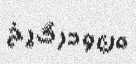
\includegraphics[]{images/3_rb.png}               &  &  \\ \cline{1-2}
\textbf{Remove distortion}      & 
\includegraphics[]{images/1_rd.png}               &  &  \\ \cline{1-2}
\textbf{Plain white background} & 
\includegraphics[]{images/0_pw.png}               &  &  \\ \cline{1-2}
\end{tabular}
\caption{Examples of synthetic data generated for each experiment. Note the high degree of pixelation; incorrectly-added spaces between characters;  the incorrect placement of some diacritics after, rather than over, characters; and that the `remove skew' data is incorrectly skewed to ten degrees.}
\label{table:synthetic_examples}
\end{table}

\begin{table}[H]
\begin{tabular}{|l|l|ll}
\cline{1-2}
\textbf{Segment}             & \textbf{Image} &  &  \\ \cline{1-2}
\textbf{Train}               & 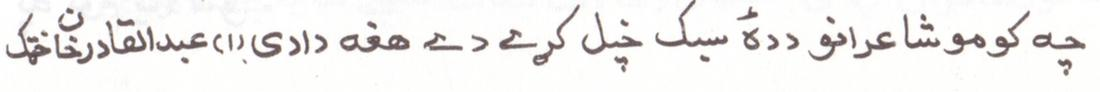
\includegraphics[width=0.7\textwidth]{images/PasPo-0066-23.jpg}             &  &  \\ \cline{1-2}
\textbf{Validation}            &  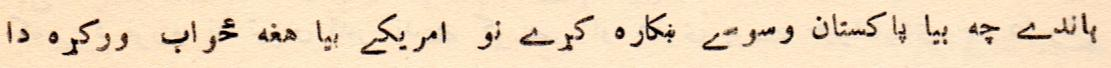
\includegraphics[width=0.7\textwidth]{images/Abasn-0002-4.jpg}              &  &  \\ \cline{1-2}
\textbf{Test}            & 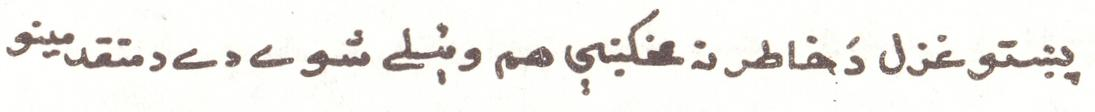
\includegraphics[width=0.7\textwidth]{images/KhKul-0003-4.jpg}               &  &  \\ \cline{1-2}
\end{tabular}
\caption{Examples of train, validation, and test data from the KPTI dataset. These have been arbitrarily chosen to demonstrate the range of books in the data.}
\label{table:kpti_examples}
\end{table}
\end{document}
